\documentclass[11pt,a4paper]{article}
\usepackage[margin=22mm]{geometry}
\usepackage{amsmath}
\usepackage{booktabs}
\usepackage{multicol}
\usepackage[most]{tcolorbox}
\usepackage{tikz}

\newcommand\OpenEvidenceColumns{\setlength{\columnsep}{18pt}\begin{multicols}{2}}
\newcommand\CloseEvidenceColumns{\end{multicols}}
\long\def\EmitCaptured#1{#1}

\begin{document}

\section{Ordinary prose and notes}

PROSEMARKA begins a long ordinary paragraph. The live preview must preserve
the exact page while a nearby character changes, then replace it with the
new exact page without making the editor wait for the whole document. This
paragraph is deliberately verbose so that line breaking, paragraph glue,
and page checkpoints all participate in the stress case. It continues with
plain words about evidence, measurement, reproducibility, and careful
comparison between an immediate view and the later certified rendering.

The second paragraph contains FOOTMARKA inside a footnote\footnote{The
FOOTMARKA annotation is long enough to wrap across several lines. Its text
is edited inside a braced command argument, but the replacement itself is
ordinary visible text and does not alter TeX grouping or control sequences.
The insertion stream must remain exact after the resumed page is shipped.}.
The surrounding body continues after the insertion and creates enough
material for TeX to make a genuine placement decision at the bottom margin.

Another paragraph fills the first page with natural language. It discusses
why latency and correctness are separate promises: the first visible result
may be local and provisional, while the page-sealed result must be identical
to a clean LuaLaTeX run. Neither promise excuses a blank preview or a stale
character that remains on screen after the exact wave has completed.

\clearpage

\section{Boxed material}

\begin{tcolorbox}[
  enhanced,
  breakable,
  colback=blue!3,
  colframe=blue!55!black,
  title={A breakable evidence box}
]
BOXMARKA appears in the first paragraph of a real tcolorbox. The box has a
painted background, border, title, internal padding, and enough content to
exercise the package's grouping and page-building hooks. Editing this text
must not demote the complete document to a synchronous full compile.

The second boxed paragraph contains an inline equation
$E=mc^2$ and more prose. It is intentionally ordinary at the edit locus even
though the enclosing environment is structurally rich. A conservative
admission rule should inspect what changed, not reject every character merely
because TeX happens to execute the environment inside a group.

The third boxed paragraph repeats the operational requirement. Show the
nearby response quickly, retain the last certified pixels outside the dirty
region, and promote the replacement only after the complete page wave is
validated. The box itself may span, but its source remains a single protected
environment block for segmentation.
\end{tcolorbox}

Text after the box verifies that the environment closed correctly and that
following paragraphs return to the normal page builder.

\clearpage

\section{TikZ and a floating figure}

The paragraph before the figure gives the float queue real surrounding text.
It also references Figure~\ref{fig:mixed-heavy}, forcing label and auxiliary
state to agree with the certified baseline.

\begin{figure}[htbp]
  \centering
  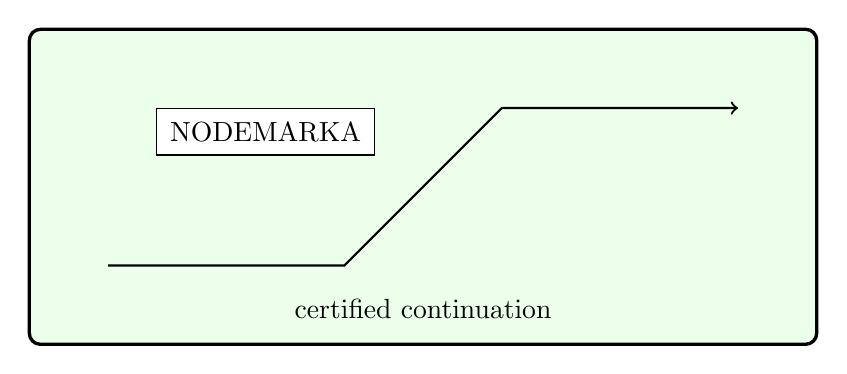
\begin{tikzpicture}[x=1cm,y=1cm]
    \draw[very thick,rounded corners,fill=green!8] (0,0) rectangle (10,4);
    \draw[->,thick] (1,1) -- (4,1) -- (6,3) -- (9,3);
    \node[draw,fill=white,inner sep=5pt] at (3,2.7) {NODEMARKA};
    \node[below] at (5,0.7) {certified continuation};
  \end{tikzpicture}
  \caption{CAPTIONMARKA describes a real TikZ float whose caption is edited
  inside a braced argument.}
  \label{fig:mixed-heavy}
\end{figure}

The text after the figure is long enough to let placement affect the page.
The checkpoint before this page must retain the earlier exact pages, while
the continuation recomputes the page containing the graphic, its caption,
the figure counter, and all remaining output. A same-length visible edit in
the node label or caption must be admitted without treating it as a change
to TikZ syntax.

\clearpage

\section{Tables and another float}

\begin{table}[htbp]
  \centering
  \begin{tabular}{lrrr}
    \toprule
    item & first & second & total \\
    \midrule
    TABLEMARKA & 12 & 18 & 30 \\
    beta       & 23 & 31 & 54 \\
    gamma      &  7 & 11 & 18 \\
    delta      & 19 & 29 & 48 \\
    epsilon    & 13 & 17 & 30 \\
    \bottomrule
  \end{tabular}
  \caption{A ruled numerical table in the float queue.}
  \label{tab:mixed-heavy}
\end{table}

This paragraph refers to Table~\ref{tab:mixed-heavy}. The rows, rules,
caption, counter, and float placement must all survive repeated edits. The
edited cell is plain text between alignment tabs, which exercises a different
parser context from both ordinary prose and braced command arguments.

An additional paragraph fills the page so that the table cannot be reduced
to a trivial isolated object. Exact convergence must include this prose and
the vertical glue around the float, not only the text extracted from the PDF.

\clearpage

\section{Macro-wrapped multicolumn material}

\OpenEvidenceColumns

COLMARKA begins the left column. The begin and end of this multicols region
are hidden behind arbitrarily named macros, so a raw environment scanner
cannot see the output-routine transition. The certified alias analysis must
keep the entire region as one structural block while still allowing a plain
character replacement to resume from the preceding exact page checkpoint.

The next paragraph adds column-balanced material. It explains that the fast
view is not an independent pagination authority. The exact continuation owns
the final column breaks, balancing, footnotes, and float interactions.

\columnbreak

The right column starts explicitly. Its prose forces the environment to use
the real multicolumn output routine rather than merely setting two short
lines. Several sentences supply line wrapping and paragraph glue. The source
remains easy to inspect even though the resulting page builder is complex.

The final column paragraph contains a small display:
\[
  \sum_{k=1}^{n} k = \frac{n(n+1)}{2}.
\]
Text follows the formula so the edit test covers a mixed page rather than a
page consisting only of ordinary glyphs.

\CloseEvidenceColumns

\clearpage

\section{Combined tail}

% COMMENTMARKA remains literal input and is a negative replay case.

The last page combines a short box, a footnote, and normal prose after all
earlier floats and multicolumn output have settled.

\begin{tcolorbox}[colback=orange!4,colframe=orange!60!black,title={Tail box}]
TAILBOXA is the final boxed marker. A late edit should replay only this tail,
not charge the user for every page that precedes it.
\end{tcolorbox}

TAILPROSEA starts the final ordinary paragraph. The closing paragraph has
TAILNOTEA in a footnote\footnote{TAILNOTEA is the
last braced visible marker in the document.} and then continues with enough
words to make the final partial page nonempty. The test checks the PDF text
after every certified wave, so accepting the source without painting the
new glyph cannot masquerade as success.

\begin{verbatim}
VERBATIMMARKA is deliberately a negative admission case.
\end{verbatim}

\clearpage

\section{Captured multi-page argument}

\EmitCaptured{
CAPTURESTARTA begins a macro argument whose entire token list is scanned
before the macro body executes. This first page of the argument contains
enough ordinary prose to make the scanner/read-ahead boundary observable.
The shipping chain must never select a checkpoint created after this unit
was requested, even when the edited marker is physically several pages
later. Replaying from the checkpoint before the complete unit is correct.

More prose fills the captured first page. It discusses input buffers, token
lists, argument scanning, and why a source coordinate alone does not prove
that TeX will read an edited byte again. The coarse unit cursor is acceptable
only because this whole balanced argument stays in one source unit.

\newpage

The middle page is still part of the same captured argument. Its paragraphs
create a real shipout after TeX has already scanned the eventual marker.
Selecting that page checkpoint would preserve the old token list and silently
ignore the new source character, which is exactly the regression this fixture
is designed to catch.

Additional middle-page prose supplies line wrapping and a stable physical
page. The exact wave may begin before this page, but it must never begin after
the source unit itself was materialized.

\newpage

CAPTUREMARKA appears on the final physical page of the captured argument.
Changing its final letter must resume from before CAPTURESTARTA, regenerate
all pages in this unit, and publish only after the complete PDF validates.
}

\end{document}
